\documentclass{ximera}
% \usepackage[utf8]{inputenc}
% \usepackage{amsmath}
% \usepackage{titling}
% \setlength{\droptitle}{-7em}  
% \usepackage{tabu}
% \usepackage{adjustbox}
% \usepackage{graphics}
% \usepackage{array}
% \usepackage{comment}
% \usepackage{harpoon}
% \newcommand{\vvec}[1]{\overrightharp{#1}}
% \newcommand{\proj}[2]{\text{proj}_{\overrightharp{#2}}\,\,\overrightharp{#1}}
% \usepackage{tikz}
% %\usetikzlibrary{angles, arrows.meta,intersections,quotes}
% \usetikzlibrary{quotes,arrows.meta,angles}




\title{Worksheet 1}
\author{Math 118: Fall 2024} 

\begin{document}

\begin{abstract}
This worksheet is NOT extra credit. It is a chance to familiarize yourself with this page and the software. 

Future worksheets (Worksheet 3 and beyond) will be counted as extra credit towards your next quiz!
\end{abstract}
\maketitle


\begin{itemize}
    \item This worksheet is supposed to prepare you for the coming quiz. There are no restrictions on the tools you may use on this worksheet. You may use your notes, you may work with classmates and the TA/proctor. 
    \item It's suggested you use a cheat sheet which is both sides of an $8.5\times 11$ sheet of paper and a scientific calculator as practice for the quiz.
    \item Please round all answers to two (nonzero) decimal places where applicable.
    \item Simplify all answers.
\end{itemize}


\noindent{\large \bf Problem 1: Foundation} (0 pts)

Consider the functions $$f(x)=\frac{2x-\sqrt{x}}{x^2+2}\qquad\text{ and }\qquad g(q)=5e^{2q}.$$

     \begin{enumerate}[label=(\alph*)]
        \item Find $f(0)$ and $f(4)$. $$f(0)=\answer[given]{0}\qquad\text{ and }\qquad f(4)=\answer[given]{1/3}$$ \vspace{5cm}
        \item Find percentage change in $f(x)$ from $x=1$ to $x=4$. \vspace{5cm}
        \item Find percentage change in $g(q)$ from $q=1$ to $q=2$. 
    \end{enumerate}
    




\newpage $\,$
\newpage


\noindent{\large \bf Problem 2: Foundation} (0 pts)

Answer each of the following.

\begin{enumerate}[label=(\alph*)]
    \item If $p$ is in units of dollars per shoe and $q$ is in units of thousands of shoes, what are the units of $pq$? \vspace{5cm}
    \item If $v$ is in units of miles per hour and $t$ is in units of minutes, what are the units of $\frac{v}{t}$? \vspace{5cm}
    \item If a taco shop lowers the price of their tacos from $\$4.00$ to $\$3.50$ find the percent change in price. 
\end{enumerate}



\newpage $\,$
\newpage


\noindent{\large \bf Problem 3: Foundation} (0 pts)

Consider the functions $f(x)$, $g(x)$, and $h(x)$.

    \begin{center}
    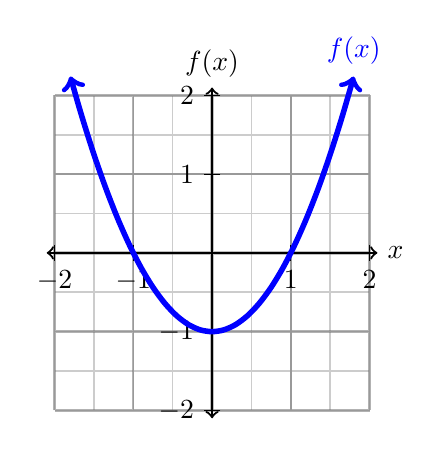
\begin{tikzpicture}
     \draw[semitransparent,step=5mm, line width=0.2mm, black!40!white] (-2,-2) grid (2,2);
\draw[semitransparent,step=5cm, line width=0.5mm, black!50!white] (-2,-2) grid (2,2);
\draw[semitransparent,step=1cm, line width=0.3mm, black!60!white] (-2,-2) grid (2,2);
        \draw[thick,<->] (-2.1,0) -- (2.1,0) node[right]{$x$};
        \draw[thick,<->] (0,-2.1) -- (0,2.1) node[above]{$f(x)$};
        \foreach \x in  {-2,-1,1,2}
    \draw[shift={(\x,0)},color=black] (0pt,3pt) -- (0pt,-3pt) node[below] 
{$\x$}; 
\foreach \y in  {-2,-1,1,2}
    \draw[shift={(0,\y)},color=black] (3pt,0pt) -- (-3pt,0pt) node[left] 
{$\y$}; 
        \draw[line width=2pt,<->, domain=-1.8:1.8, smooth, variable=\x, blue] plot ({\x}, {(\x)^2-1}) node[above] {$f(x)$};
    \end{tikzpicture}
    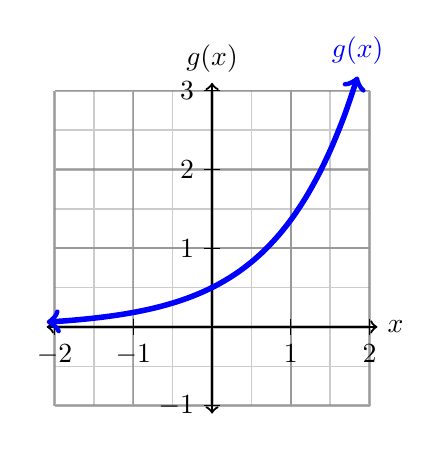
\begin{tikzpicture}
     \draw[semitransparent,step=5mm, line width=0.2mm, black!40!white] (-2,-1) grid (2,3);
\draw[semitransparent,step=5cm, line width=0.5mm, black!50!white] (-2,-1) grid (2,3);
\draw[semitransparent,step=1cm, line width=0.3mm, black!60!white] (-2,-1) grid (2,3);
        \draw[thick,<->] (-2.1,0) -- (2.1,0) node[right]{$x$};
        \draw[thick,<->] (0,-1.1) -- (0,3.1) node[above]{$g(x)$};
        \foreach \x in  {-2,-1,1,2}
    \draw[shift={(\x,0)},color=black] (0pt,3pt) -- (0pt,-3pt) node[below] 
{$\x$}; 
\foreach \y in  {-1,1,2,3}
    \draw[shift={(0,\y)},color=black] (3pt,0pt) -- (-3pt,0pt) node[left] 
{$\y$}; 
        \draw[line width=2pt,<->, domain=-2.1:1.85, smooth, variable=\x, blue] plot ({\x}, {exp(\x)/2}) node[above] {$g(x)$};
    \end{tikzpicture}    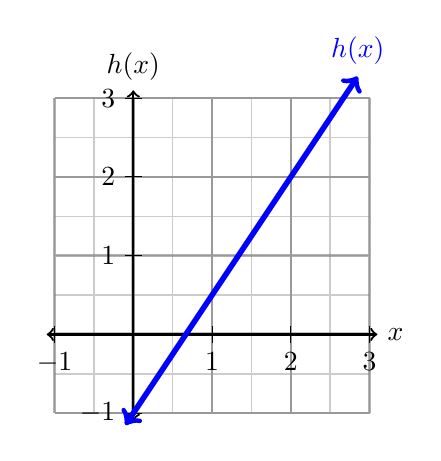
\begin{tikzpicture}
     \draw[semitransparent,step=5mm, line width=0.2mm, black!40!white] (-1,-1) grid (3,3);
\draw[semitransparent,step=5cm, line width=0.5mm, black!50!white] (-1,-1) grid (3,3);
\draw[semitransparent,step=1cm, line width=0.3mm, black!60!white] (-1,-1) grid (3,3);
        \draw[thick,<->] (-1.1,0) -- (3.1,0) node[right]{$x$};
        \draw[thick,<->] (0,-1.1) -- (0,3.1) node[above]{$h(x)$};
        \foreach \x in  {-1,1,2,3}
    \draw[shift={(\x,0)},color=black] (0pt,3pt) -- (0pt,-3pt) node[below] 
{$\x$}; 
\foreach \y in  {-1,1,2,3}
    \draw[shift={(0,\y)},color=black] (3pt,0pt) -- (-3pt,0pt) node[left] 
{$\y$}; 
        \draw[line width=2pt,<->, domain=-0.1:2.85, smooth, variable=\x, blue] plot ({\x}, {3*\x/2-1}) node[above] {$h(x)$};
    \end{tikzpicture}
    \end{center}

    \begin{enumerate}[label=(\alph*)]
        \item Write the points where $f(x)=0$. \vspace{1cm}
        \item\makebox[0pt][r]{(1 pt) \hspace{0.65cm}} Which of the following could be $f(x)$? \textit{Hint: Find $f(0)$ and $f(1)$ for each.} 
        \begin{enumerate}
            \item[(A)] $f(x)=-x^2+1$
            \item[(B)] $f(x)=-x^2-1$
            \item[(C)] $f(x)=x^2+1$
            \item[(D)] $f(x)=x^2-1$
        \end{enumerate}
        \item What is $g(0)$? \vspace{3cm}
        \item\makebox[0pt][r]{(1 pt) \hspace{0.65cm}} Is $g(x)$ increasing or decreasing? \vspace{1cm}
        \item Knowing $h(x)$ linear, find the equation for $h(x)$.  
    \end{enumerate}

\newpage $\,$
\newpage


\noindent{\large \bf Problem 4: Foundation} (0 pts)

Graph each of the following on the appropriate graph.

    \begin{center}
    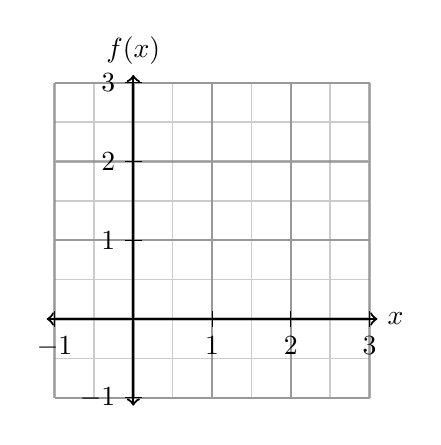
\begin{tikzpicture}
     \draw[semitransparent,step=5mm, line width=0.2mm, black!40!white] (-1,-1) grid (3,3);
\draw[semitransparent,step=5cm, line width=0.5mm, black!50!white] (-1,-1) grid (3,3);
\draw[semitransparent,step=1cm, line width=0.3mm, black!60!white] (-1,-1) grid (3,3);
        \draw[thick,<->] (-1.1,0) -- (3.1,0) node[right]{$x$};
        \draw[thick,<->] (0,-1.1) -- (0,3.1) node[above]{$f(x)$};
        \foreach \x in  {-1,1,2,3}
    \draw[shift={(\x,0)},color=black] (0pt,3pt) -- (0pt,-3pt) node[below] 
{$\x$}; 
\foreach \y in  {-1,1,2,3}
    \draw[shift={(0,\y)},color=black] (3pt,0pt) -- (-3pt,0pt) node[left] 
{$\y$};
    \end{tikzpicture}
    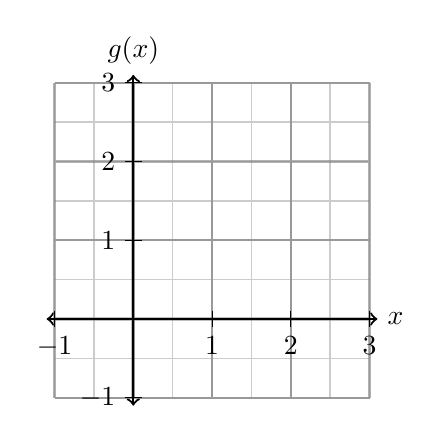
\begin{tikzpicture}
     \draw[semitransparent,step=5mm, line width=0.2mm, black!40!white] (-1,-1) grid (3,3);
\draw[semitransparent,step=5cm, line width=0.5mm, black!50!white] (-1,-1) grid (3,3);
\draw[semitransparent,step=1cm, line width=0.3mm, black!60!white] (-1,-1) grid (3,3);
        \draw[thick,<->] (-1.1,0) -- (3.1,0) node[right]{$x$};
        \draw[thick,<->] (0,-1.1) -- (0,3.1) node[above]{$g(x)$};
        \foreach \x in  {-1,1,2,3}
    \draw[shift={(\x,0)},color=black] (0pt,3pt) -- (0pt,-3pt) node[below] 
{$\x$}; 
\foreach \y in  {-1,1,2,3}
    \draw[shift={(0,\y)},color=black] (3pt,0pt) -- (-3pt,0pt) node[left] 
{$\y$};
    \end{tikzpicture}    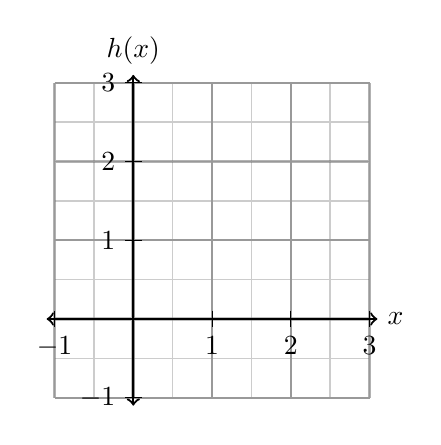
\begin{tikzpicture}
     \draw[semitransparent,step=5mm, line width=0.2mm, black!40!white] (-1,-1) grid (3,3);
\draw[semitransparent,step=5cm, line width=0.5mm, black!50!white] (-1,-1) grid (3,3);
\draw[semitransparent,step=1cm, line width=0.3mm, black!60!white] (-1,-1) grid (3,3);
        \draw[thick,<->] (-1.1,0) -- (3.1,0) node[right]{$x$};
        \draw[thick,<->] (0,-1.1) -- (0,3.1) node[above]{$h(x)$};
        \foreach \x in  {-1,1,2,3}
    \draw[shift={(\x,0)},color=black] (0pt,3pt) -- (0pt,-3pt) node[below] 
{$\x$}; 
\foreach \y in  {-1,1,2,3}
    \draw[shift={(0,\y)},color=black] (3pt,0pt) -- (-3pt,0pt) node[left] 
{$\y$}; 
    \end{tikzpicture}
    \end{center}

    \begin{enumerate}[label=(\alph*)]
        \item $f(x)$ where $f(x)=-\frac{2}{3}x+2$. \vspace{1cm}
        \item $g(x)$ where $g$ is the line with slope $\frac{1}{2}$ and goes through the point $(0,1)$. \vspace{1cm}
        \item What is the equation of the line $g(x)$? \vspace{4cm}
        \item $h(x)$ where $h(x)$ is the line through $(-1,-1)$ and $(3,2)$. \vspace{1cm}
        \item What is the equation of the line $h(x)$?
    \end{enumerate}

\newpage $\,$
\newpage



\end{document}